\subsection{Design}

Formålet med dete kapitel er at planlægge løsningen, ud fra de krav der der er
stillet, sammenholdt med erfaringerne fra analysen.

%Skal indeholde Overvejelser, beslutninger og resultater vedr.
%Softwarearkitektur og detaljeret design, herunder design af persistens. 

\subsubsection{Trelagsarkitektur}%
\label{ssub:3_lags_arkiteturen}
%i denne sektion beskrives vores tre-lags arkitektur.
%Lokalisering af ændringer

Kravet om en trelagsarkitektur (IF-01) er markeret om et "must" i prioriteringen af
krav. I FURPS+ analysen er kravet placeret som en "Design constraint", da dette
stiller et krav til designet af systemets arktitektur. 

%Hvordan kan lagene separeres? 

\paragraph{Interfaces} Et oplagt værktøj til at opdele lagene i
trelagsarkitekturen er anvendelse af interfaces. Med interfaces i mellem lagene 
skal hver enkelt lag kun afhænge af det specificerede interface. På denne måde
er der ingået en \emph{kontrakt} i mellem de to pågældende lag.
Ved anvendelse af disse interfaces behøves det lag der anvender interfacet ikke
at kende til selve implementatationen af interfacet.

\paragraph{Implementering af trelagsarkitekturen}%
\label{par:implementering_af_trelagsarkitekturen}

Et designmønster der der er en oplagt del af trelagsarkitekturen er
designmønsteret 'Model-View-Controller'. Dette designmønster er struktureret
således:

\renewcommand{\baselinestretch}{1}
\begin{figure}[H]
    \centering
    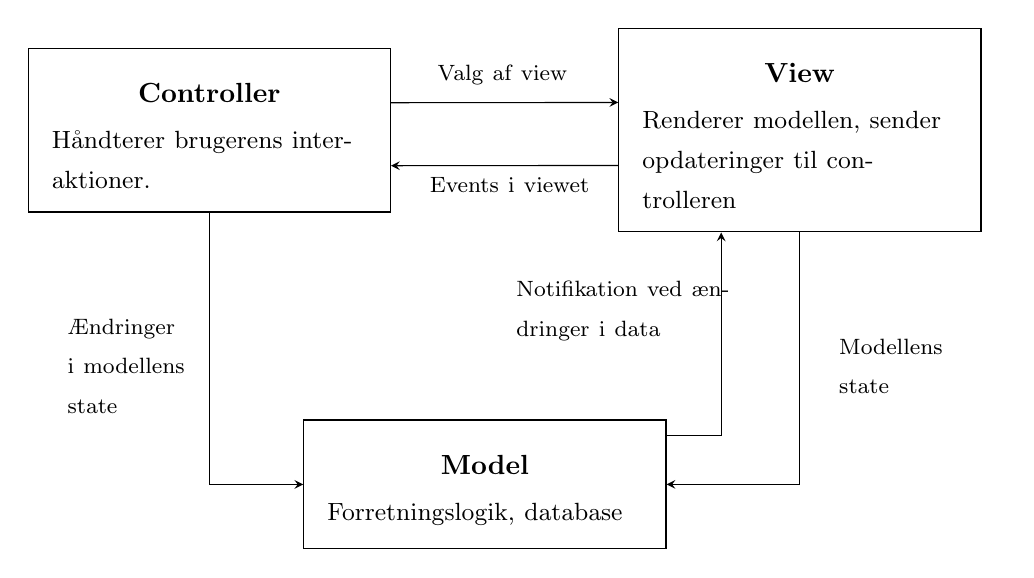
\begin{tikzpicture}
        \node[rectangle, draw, text width=4cm, inner sep=3mm] (view) at (7.5,0) 
            { \vspace{-4mm}\begin{center}
                    \textbf{View}
                \end{center}
            %\hline
            \vspace{-2mm} \small
             Renderer modellen, sender opdateringer til controlleren};
        \node[rectangle, draw, text width=4cm, inner sep=3mm] (controller) at
            (0,0) 
            { \vspace{-4mm}\begin{center}
                    \textbf{Controller}
                \end{center}
            %\hline
            \vspace{-2mm} \small
            Håndterer brugerens interaktioner.};
        \node[rectangle, draw, text width=4cm, inner sep=3mm] (model) at
            (3.5,-4.5) 
            { \vspace{-4mm}\begin{center}
                    \textbf{Model}
                \end{center} \small
            %\hline
            \vspace{-2mm}
            Forretningslogik, database};
        \node[text width=3cm] (nodetoview ) at (4.4, 0.7) {\footnotesize{Valg af view}};
        \node[text width=3cm] (tocontroller) at (4.3, -0.7) {\footnotesize{Events i viewet}};
        \node[text width=3cm] (nodetoview ) at (5.4, -2.3) {\footnotesize{Notifikation ved ændringer i data}};
        \node[text width=2cm] (modeltoview ) at (9, -3) {\footnotesize{Modellens state}};
        \node[text width=2cm] (controllertomodel ) at (-0.8, -3) {\footnotesize{Ændringer i modellens state}};
        \draw[-stealth] ([yshift= -0.7cm]controller.north east) -- ([yshift= -0.95cm]view.north west);
        \draw[stealth-] ([yshift= -1.5cm]controller.north east) -- ([yshift= -1.75cm]view.north west);
        \draw[-stealth] ([yshift= -0.2cm]model.north east) -| ([xshift= -1cm]view.south);
        \draw[stealth-] (model.east) -| (view.south);
        \draw[-stealth] (controller.south) |- (model.west);
    \end{tikzpicture} 
    \label{fig:mvc}
\end{figure}
\renewcommand{\baselinestretch}{1.2}

Dette designmønster separerer interaktion of præsentation fra systemets data.
View observerer data der holdes i model. View præsenterer det data der holdes i
model til brugeren. Controlleren står for at respondere på der sker i view, fx
hvis en bruger klikker på et element der skal starte et nyt view, da står den
for det sætte det nye view til at blive vist. Den står også at håndtere hvad der
gøres på selve klikket. 
Modellen repræsenterer de to andre lag, forretningslogiklaget og persistenslaget.
\paragraph{Pakkediagram} Systemet er delt op i pakker efter præsentations-,
domæne- og persistenslag. Ved denne opdeling kan det nemmere sikres at
trelagsarkitekturen overholdes. Et pakkediagram blev opsat og kan ses på figur
\ref{fig:PackageDiagram}

\begin{figure}[H]
    \centering
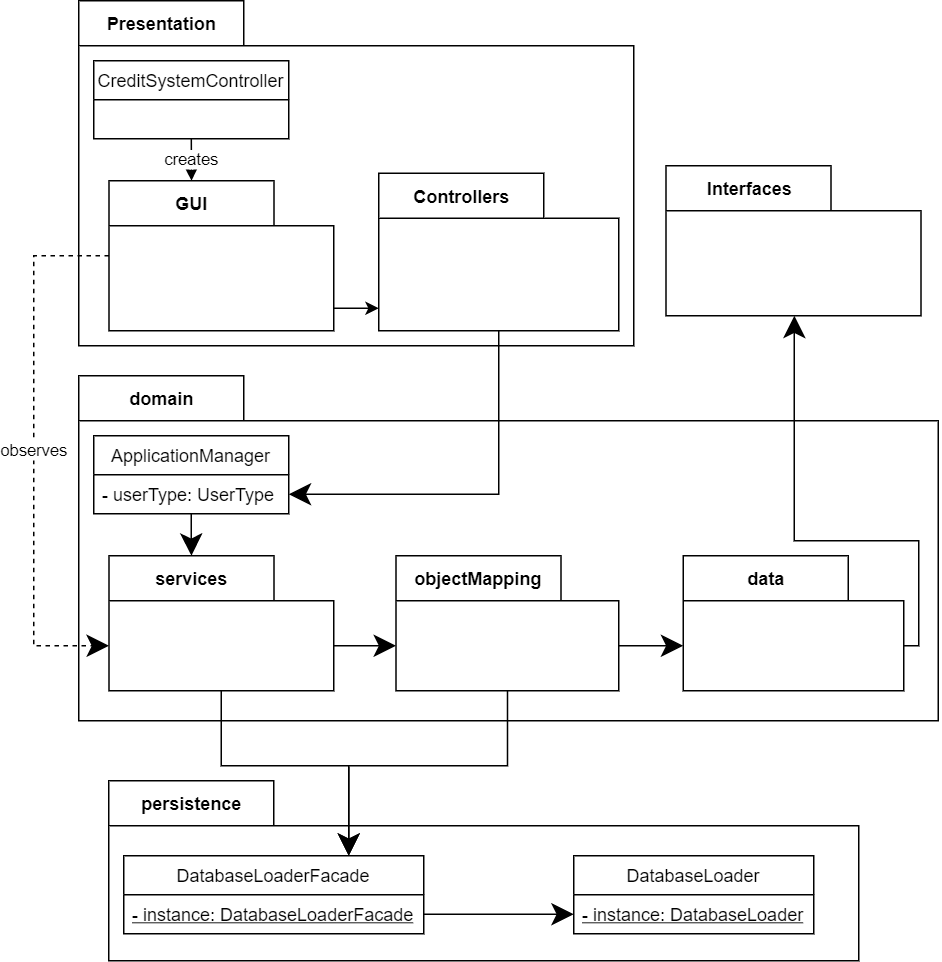
\includegraphics[scale = 0.3]{images/PackageDiagram.png}
    \caption{Pakkediagram for systemet}
    \label{fig:PackageDiagram}
\end{figure}

Figur \ref{fig:PackageDiagram} viser hvordan pakkerne kommunikerer med hinanden.
Klassen CreditSystemController, viser en GUI for brugeren. Når brugeren
foretager en handling, knytter GUI sig til nogle controllers i pakken
Controllers som kalder metoder på ApplicationManager i domænelaget.
ApplicationManager kalder den passende Manager i pakken Services som kan gøre en
af to ting: 

\begin{itemize}
    \item Hvis brugeren har oprettet en ny kreditering i GUI er objektet
        allerede instantieret, og manageren kalder derfor en 'put' metode på
        DatabaseLoaderFacade i persistensLaget, som derefter kalder den passende
        metode i DatabaseLoader.  
    \item Hvis brugeren har søgt efter en
        kreditering, kalder manageren først pakken objectMapping, som herefter
        kalder en
    \item Hvis brugeren har oprettet en ny kreditering i GUI er objektet allerede instantieret, og manageren kalder derfor en 'put' metode på DatabaseLoaderFacade i persistensLaget, som derefter kalder den passende metode i DatabaseLoader. 
    \item Hvis brugeren har søgt efter en kreditering, kalder manageren først pakken objectMapping, som herefter kalder en 'get' funktion på DatabaseLoaderFacade som dernæst kalder den passende metode på DatabaseLoader der queryer databasen, og returnerer resultaterne. Disse resultater får objectMapping pakken, og instantierer objekter via data pakken i domain.
\end{itemize}



\subsubsection{Klassediagram}%
\label{ssub:klassediagram}


\subsubsection{Systemsekvensdiagrammer}%
\label{ssub:systemsekvensdiagrammer}

